\chapter{Case Study: ENBU 79X/89X Industry Project \label{ch6}}

The objective of this chapter is to explore in detail the case study selected to assess the learning design that guided the implementation of \emph{WorkshopAR}. The
Industry Project course offered an ideal scenario to evaluate the collaborative premise behind all the proposals at the core of this research, being a course guided by
strong teamwork and communication requirements.

The complexity of the course also opened the opportunity to analyse several factors that were not initially considered in the methodological design. Thanks to the open
nature of the project and all the different profiles present among the students, the observations of the usage of \emph{WorkshopAR} were able to capture interesting
scenarios about the consolidation of teams and the variety of resources used by students to fulfil their academical goals. The teaching staff was also incorporated into
the observation process, adding a distinct perspective to the use of \emph{WorkshopAR} in the classroom and the implementation of collaborative approaches for teaching.

Section \ref{sec:6-1} will first provide an overview of the Industry Project course, its general design and learning goals, as well as the philosophy guiding that design
as it could be inferred from the material available and the conversations held with the teaching staff.

Sections \ref{sec:6-2} and \ref{sec:6-3} will detail the learning design process used for the development of \emph{WorkshopAR} based on the goals proposed in section
\ref{sec:3-1-1-3}, how the different functionalities developed achieved the proposed goals and the different activities integrated into the Industry Project course.

Sections \ref{sec:6-4} to \ref{sec:6-8} will present the main content of the case study, recounting the development of the course through twenty weeks of observations. The
structure of the case allowed to organise the data in four major milestones, first described within the point of view of the course, followed by the intervention done with
\emph{WorkshopAR}, allowing for preliminary analysis and reflection for each milestone.

Finally, sections \ref{sec:6-9} and \ref{sec:6-10} will offer a description and analysis of the overall experience from the point of view of the students and the teaching
staff based on the data obtained from the complementary research instruments such as interviews and questionnaires; followed by the final conclusions in section \ref{sec:6-11}.

\section{Description and Design of ENBU 79X/89X Industry Project \label{sec:6-1}}

Industry Project is a last-year course offered by the School of Built Environments at \ac{AUT}. The course offers students of the Architectural Design, Construction Engineering,
Construction Management and Quantity Surveillance programmes the opportunity to experience a multidisciplinary project that emulates the procedures and circumstances often
found in the construction industry.

Simulation is one of the key components behind the design of the course. Acting as a capstone course for several of the programmes that the School of Built Environments
offers, the main goal is to expose the students to many of the scenarios and procedures commonly found in a construction project, while emulating several of the roles and
tasks that need to be present in an architectural design or construction management firm.

The course covers little to no actively taught material, relying instead on the information covered in previous years. The learning goals focus more on providing a hands-on
experience through challenges and scenarios that could be found in real-life projects, promoting the development of the skills necessary for the design, communication and
planification of a solution, as stated by the course goals:

\begin{itemize}
    \item Propose, organise, design, analyse, execute, and reflect on a multi-disciplinary project.
    \item Apply existing construction and engineering knowledge and skills to the project.
    \item Conduct a systematic literature review to identify works previously undertaken and gaps requiring research.
    \item Demonstrate initiative and independence in decision making where appropriate.
    \item Present project progress and technical details to multi-disciplinary audiences.
    \item Deliver and present comprehensive client reports at relevant professional standards.
\end{itemize}

The learning goals of the course align with the ideas promoted trough the learning intervention with \emph{WorkshopAR} in key aspects like decision-making, communication,
and multi-disciplinary, multiuser work. Industry Project offers the opportunity to apply the knowledge and skills that the students have gathered through their career in a
situation that requires the collaboration with other professionals to fulfil the goals of the project.

The methodology of the course helps the students in the development of the project through three main mechanisms: the client simulation, weekly workshops, and open work
sessions. These three elements feed on each other to help the students immerse in the development of the project in a way that simulates real work experience. This
simulation involved a substantial effort of creating the context of the project with the help and input of several professionals, both part of the faculty and from
external sources. The project asked the students to analyse:

\begin{itemize}
    \item Geotechnical data of the terrain to be developed.
    \item Cultural, economic, and social factors of the zone where the site is located.
    \item Requirements and proposals from the client.
    \item Requirements and proposals from other stakeholders like the local community and the government.
\end{itemize}

The fictional client is represented by several experts, most of them part of the faculty but not of the teaching staff, referred to as Task Leaders. They are available to
answer questions about their requirements for the project and about the work expected from each of the four roles present in the course. Additionally, each group would act
as a task team in charge of the design and management of the development of the construction project. ENBU 79X/89X acts as the capstone for four different programs, and
each group had at least one representative of each role: \ac{AE}, \ac{CE}, \ac{CM} and \ac{QS}. The group was expected to coordinate efforts to create a coherent proposal
for the construction project, while fulfilling specific tasks and deliveries specific for each role. Finally, the group had to provide weekly and milestone reports to the
client, communicating the state of the project, the creative decisions made, and the management process proposed to oversee the construction.

The course relies entirely on the project approach to address the learning outcomes. There is no taught content in the course for any of the roles, relying more on access
to material of previous courses and curated information on the web, all through the \ac{LMS} used for the course. A second support tool for the technical content is the
presence of the Task Leaders, who can be consulted about the requirements for each role, for feedback about the work done or for recommendations on how to complete the
deliveries.

The main approach used by the course to convey course content to the students is through the weekly workshops. These take two possible forms: workshops guided by the
teaching staff, which are meetings used to clarifying aspects of the project, or workshops guided by external professionals, used to talk about subjects useful for
professional development, like team management techniques and current trends in the industry.

The final methodological implementation of the course are the open work sessions, which represent most of the time spend by the students in the course. As the name suggest,
they are open in nature, allowing the students to use the time in the classroom (about two sessions of 1 hour per week, depending on the length of other activities) to
meet with their group or with other students to organise their work and progress towards the competition of the different deliverables. These sessions also allow the
students to have direct access to the teaching staff and a somewhat reliable access to their peers.

The assessment of the course is completely individual. Deliverables and the proposed solution to the project are built as a group, but at the end, each student presents
their own contribution. The main assessment tools are oral presentations and client reports. The presentations consist of short 5-minute poster expositions about the
overall proposal of the group for the project, the current state of development and the personal contributions of the students in that proposal. There are two oral
presentations along the course, one focused on the architectural design and the other on the final proposal.

The client reports consist of weekly formative assessment of the group's progress and two final reports at the end of each semester. The biweekly reports are not marked
but are analysed weekly to give feedback to the students about issues found in the reports. It is also a useful tool to identify the overall progress of all the groups and
to take decisions on how to manage due dates and marking expectations. The final report is marked and consists of a quick summary of the personal contributions of each
student to the project, as well as a reflection of the work done by the group, the problems found and the steps taken to solve them.

As for the content of the project itself, it is meant to cover activities for each of the roles of the course. The specifics of the content of the project are not that
necessary for the analysis of this case study, but overall, the students must propose a solution for:

\begin{itemize}
    \item An architectural design for a building complex that considers the geotechnical data of the construction site, the functional necessities of the project and the
    complications and peculiarities found in the selected site.
    \item A construction plan that considers building materials, functional necessities and local regulations.
    \item A detailed schedule for the management of the construction, considering aspects like budget, necessary contractors, needed studies and the impact on the local
    community.
    \item A detailed consideration of the local construction requirements, the legal implications of the design and external factors like the economic and ecological
    impacts of the proposal, as well as the consideration needed related to the Waitangi treaty.
\end{itemize}

It is important to remark that all these objectives are evaluated on two fronts. First, the work done by the group, how information flows across the different roles, and
how work is coordinated to create a coherent proposal. This aspect is mostly assessed through the oral presentation. The second front is the individual contribution and
performance of each student, marked mostly by the accuracy and quality of the tasks completed, and evaluated through the final client report.

\section{WorkshopAR Learning Design \label{sec:6-2}}

This section seeks to elaborate on the information presented in Section \ref{sec:3-3-1-3} about the structure of the learning design for the project, how \emph{WorkshopAR}
approaches the learning goals proposed, and how these goals are integrated with the structure of the Industry Project course.

LO1 establishes that the students can plan their \emph{work session} by analysing the current state of their work and determining clear goals to achieve during the
session. \emph{WorkshopAR} supports this strategy by linking the creation of the \emph{digital room} with the definition of a goal for the \emph{work session}. It also
helps by distributing the activity among the participants and associating current tasks with the profile of each of them.

Observations related to LO1 can go beyond just checking if the students are defining goals and tasks during the configuration of the session or not. It could be possible
to check the level of detail applied to the definition of goals, to check if the tasks were updated along the progress of the session or if a similar analysis of the goals
or progress of work was done outside \emph{WorkshopAR}.

LO2 is related to the execution of effective collaboration and can be evidenced by using the criteria identified in the literature and explained in Sections \ref{sec:2-1-4}
and \ref{sec:2-1-5}. It is of particular interest for this project and for the overall evaluation of \emph{WorkshopAR} to see if any of the tools provided, especially
those associated with the interaction with the play models and annotations, help in creating the structures identified as useful for effective collaboration such as a free
flow of information, accountability, quality assurance and mutual dependence.

For LO2, it is also interesting to observe the types of collaboration being used by the students as described by \textcite{salmons_2019}, and if \emph{WorkshopAR} was
promoting or helping in the development of a particular form of collaboration. In general, the digital space created by \emph{WorkshopAR} would facilitate activities of
co-creation, by allowing the testing and record of ideas for the architectural design, and of transfer activities, by offering visuals that can be used to explain concepts,
decisions or design proposals.

LO3 keeps the idea of effective structures for collaboration but focuses entirely on how the group manages internal and external communication. The debate feature of
\emph{WorkshopAR} is the obvious implementation build specially to cover this learning objective, which at the same time helps the group to create an instance of dialogue,
defined by Salmons as the type of structured conversation that best promotes and executes collaboration. Observations will also search for other aspects of the tool that
promote conversation instead, the unstructured type of communication used more to foster relationships in the group.

Finally, LO4 evaluates how the group proposes and organises structured review. \emph{WorkshopAR} does not dedicate one functionality to support this learning objective,
relying more on the use of all the previously mentioned use cases to offer a structured evaluation of a design proposal, of feedback received from the client or to
organise the work needed to create the final reflection of the project.

\emph{WorkshopAR} takes into consideration the design of Industry Project and is meant to help the students to tackle the course's objectives related to effective
communication and the coordination of tasks. Figure \ref{fig:6-1} shows an ideal flow of activities during the development of a classroom session, which incorporates the
main activities proposed in the course design (class housekeep, weekly workshops, open work sessions) with an idealised version of a \emph{work session}  that a group
could perform while using \emph{WorkshopAR}.

\begin{figure}
    \centering{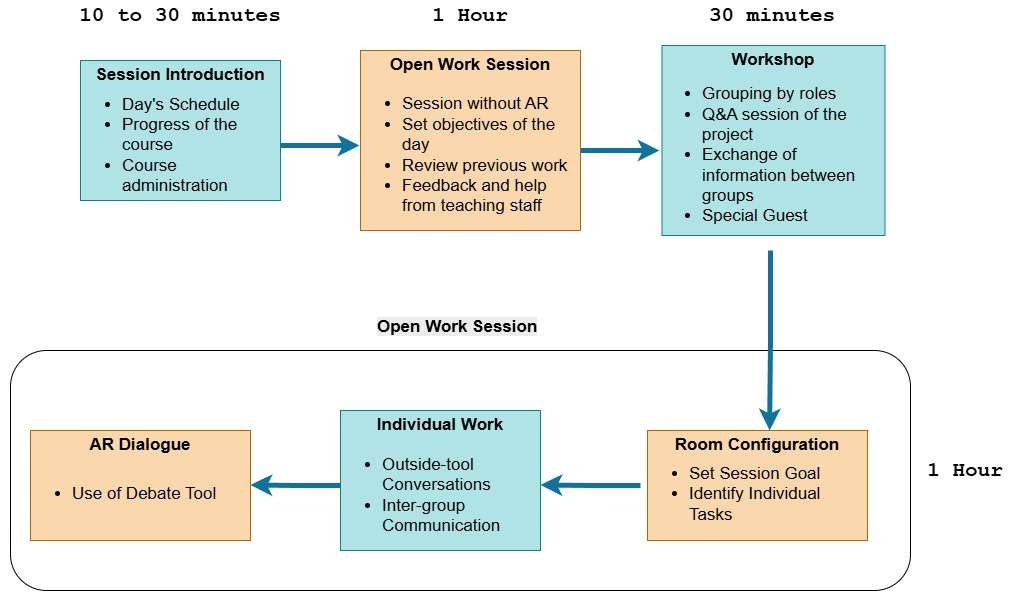
\includegraphics[alt={Figure 6.1},width=0.99\textwidth]{figures/F6-1.jpg}}
    \caption{Flow of Activities in a Classroom Session \label{fig:6-1}}
\end{figure}

This learning design is also informed by other aspects found in the literature about effective collaborative learning and the approaches taken by other projects in similar
context. Section \ref{sec:2-1-4} details some important barriers that impede a good flow of collaboration in the classroom. Two of the ideas mentioned resonated the most
with the characteristics found in the Industry Project course:

\begin{itemize}
    \item Power imbalance among the members of a group.
    \item Difficulties transferring knowledge between students.
\end{itemize}

Issues of power imbalance are inherent to any social activity \parencite{essabbar_2016}, and it was identified that the role structure proposed for the project could
promote substantial differences among the students. In the same way, \emph{WorkshopAR} proposes a very structured approach to collaboration, encouraging the students to
assign roles and to distribute tasks according to what have been discussed. A central objective of the observation process will be to identify positive and negative
behaviours derived from this design implementation, and course correct the implementation of the software if needed.

Knowledge flow in project-based approaches is also an issue that have been discussed in the past \parencite{kogtikov_2016,granado-alcon_2020,shpeizer_2019}. A possible
barrier for any group in the course could be issues communicating and transferring knowledge, considering that every role in the group has a distinct set of abilities and
approaches the project in a slightly different way, yet the project needs a coherent and unified proposal. \emph{WorkshopAR} can act in this situation as a facilitator for
the transference of knowledge, helping by offering visual tools to better convey ideas, using the space and context of the work to facilitate conversation and serving as a
visual repository of the ideas and decisions discussed among the students.

A final design consideration is the integration of the \ac{CoP} framework in the design of \emph{WorkshopAR}. As discussed in Section \ref{sec:2-1-2}, it is detrimental for
a \ac{CoP} to force its development, and effective communities thrive when formed naturally and providing the resources needed to grow. It has been proposed that a \ac{CoP}
in the classroom is better represented in the effort done by the students themselves to organise and work towards the learning objectives. Due to the nature of this
project-based course, it is possible that some of the characteristics of a \ac{CoP}, like instances of peripheral learning and a culture of self-reflection, could be
observed among the students, and \emph{WorkshopAR} could be used in these circumstances as part of the knowledge that the community is creating, as a medium to transfer
that knowledge or as a facilitator for the communication process of the community.

\section{Protocol \label{sec:6-3}}

The case study was developed in three distinct stages with different set of objectives in mind. All three stages were meant to collect descriptive data about the
development of the course, either to create a better picture of the context in which the course was happening, to gather descriptive data about the progress of the project
or to ask for more granular opinions from the students and the teaching staff, all these with the goal in mind of creating a rich recount of the course.

\subsection{Physical Documentation \label{sec:6-3-1}}

Most of the written material was accessible for the teaching staff and the students through the \ac{LMS} supporting the course. The \ac{LMS} was the primary communication
method used by the teaching staff, besides direct announcements at the beginning of a session. Students would find all the basic information about the project and the
different deliveries of the course in the \ac{LMS}, and it became the main repository for the different forms and documentation needed for the coursework, such as client
reports, presentation formats and assessment rubrics. Information about the structure, learning goals and methodology of the course was also found here. This information
was used mostly to build a good understanding of the objectives and background of the course, as well as to establish a good idea of the work expected from the students.

Although most of the assessment tools of the course consisted of oral presentations, a good amount of material had to be submitted through the LMS, either as its own
assessment or as a complement to the oral presentations. A lot of this material consisted of individual work and allowed for an interesting analysis of how the students
were organising their work as part of the group activities.

Finally, the \ac{LMS} portal also offered a discussion forum for the students meant to be the main communication channel between the students and the teaching staff
outside the classroom. Activity here was almost non-existent before the semester break, and students only started to use it after the adjustments done to the course during
the second semester. Following sections will detail this situation better, as it is an important point of analysis of the course and of the way technology is used in the
classroom for communication.

\subsection{Classroom Observations \label{sec:6-3-2}}

The main source of data coming from the case study was the direct observation of students along the classroom activities each week. This is already a departure from the
original methodology, which proposed observations of the groups outside of the classroom. It was evident during the first weeks of the semester that the students were
using mostly the classroom time for their groupwork, opting for individual work outside the classroom and for asynchronous communication with their teammates. This
situation called for some of the mechanisms of the observation process to change and adapt to what the students where really doing, but the general approach and goals for
this stage were the same.

There were three main types of observations that composed most of the data collected. All types focused on describing in as much detail as possible the type and objectives
of the activities being observed, the outstanding characteristics of the students participating and any relevant information about the background that was possible to
collect. All observations were recorded using mostly personal notes and video recordings when it was possible to do it without disrupting the classroom too much.

The first type of observations was of general activities for the whole classroom, guided normally by the teaching staff or by a guest speaker. These activities included
all the students and were not directly related to groupwork, although they often required the students to group based on their assigned roles.

These observations were useful for understanding the general structure and dynamics of the course, especially those relations between the teaching staff and the students.
These activities were often used to deal with general questions from the students, for the administration of the course and to observe the different workshops held
throughout the semester.

The initial categorisation of themes for these observations was very general:

\begin{itemize}
    \item Guidelines from the teaching staff to the students about teamwork and collaboration.
    \item Feedback given to the students about an activity or a material produced for the project.
\end{itemize}

The second type of observations was of the general groupwork performed by the students. These \emph{work sessions} often involved more than one group at a time, and the
focus was on gathering information with minimal intervention, sometimes asking quick questions to clarify a situation or to get a better idea of the context.

These observations helped in identifying the general dynamics of the groups, and the activities being completed for the project. They also constituted the baseline
observations for those activities that were not using the \ac{AR} tool and became the main point of comparison with the other observations.

Initial categorisation here was more varied. In one hand there was a group of themes searching for the collaborative strategies being used by students:

\begin{itemize}
    \item Activities and resources to organise and manage the team.
    \item Recurrent roles (beside the project's roles) and relationships being created among the students.
    \item Mechanisms to take decisions and resolve conflicts.
\end{itemize}

A second focus was the use of technology and trying to identify tendencies about what activities were mediated by digital tools:

\begin{itemize}
    \item Technologies used to produce content and fulfil learning objectives.
    \item Technologies used to access and consume content to create and/or transmit knowledge.
    \item Technologies used to mediate or facilitate communication and social relations.
\end{itemize}

The third and final type of observations were of the instances in which \emph{WWorkshopAR} was used in the activities of a group and if it was changing in some way previously
observed behaviours or promoting new ones:

\begin{itemize}
    \item Instances in which a problem was solved using \emph{WWorkshopAR}.
    \item Instances in which a problem was created because of the use of \emph{WWorkshopAR}.
    \item Behaviours promoted using \emph{WWorkshopAR}.
    \item Social activities taking place within the digital space of \emph{WWorkshopAR}.
\end{itemize}

These observations were more guided, prompted mostly by the researcher, asking the students to explore one or two features from the software, asking for feedback and
identifying instances in which the tool was used or mentioned without prompt.

\subsection{Unstructured Interviews \label{sec:6-3-3}}

The final dataset comes from unstructured interviews conducted with a random sample of the students and of the teaching staff. Both interviews focused on gathering
information about how participants saw collaboration as part of the development of the course, how do they perceive their own collaboration skills and how the course was
helping them to develop or improve those skills.

The interviews with students focused more on trying to reconstruct the team dynamics of those groups that were not directly observed, asking questions about activities
done to fulfil the requirements of the course, rules or decisions taken to manage the group and how effective did the students found those elements.

The interviews for the teaching staff were one-to-one conversations about what they perceived as effective collaboration and how did they evidence, if at all, those ideas
in the work done by the groups in the course. These interviews were used to gather information about the development of the current cohort of the course, the challenges
and complexities in managing the course and more personal opinions on the quality of the student's work and what could be done to improve the course in general.

Appendix \ref{appendix:c} of this document shows the script used for each interview.

With the learning objectives of \emph{WorkshopAR} detailed, clear mechanisms proposed for the students to fulfil those goals and the documentation of all the types of
observations proposed, the next set of sections will now recount and analyse the execution of the Industry Project course.

\section{Weeks 1 to 4: Team Consolidation \label{sec:6-4}}

The first weeks of the course were characterised by a period of accommodation. The Industry Project course offers a unique experience, and although the students at this
point have already experienced project-based approaches in the past, none had been in such a multidisciplinary context, nor with such an emphasis on simulating a
professional setting.

For the activities with \emph{WorkshopAR}, it was also a period of introduction, letting the students familiarise with the dynamics of the course before adding the extra
layer of complexity that of the observations and the usage of the software.

\subsection{General Observations \label{sec:6-4-1}}

Classroom sessions took place on Friday mornings across two big arrangeable lecture rooms, needed to accommodate the approximately eighty students enrolled. The space
provided several tables that could be moved, separated, or merged to create different configurations, ideal for the dynamic groupwork that the course was relying the most
on. The rooms also enabled the constant flow of people and activities present in one session, as described in Section \ref{sec:6-3}, and provided ample space for each group
to work comfortably using their personal equipment.

\begin{figure}
    \centering{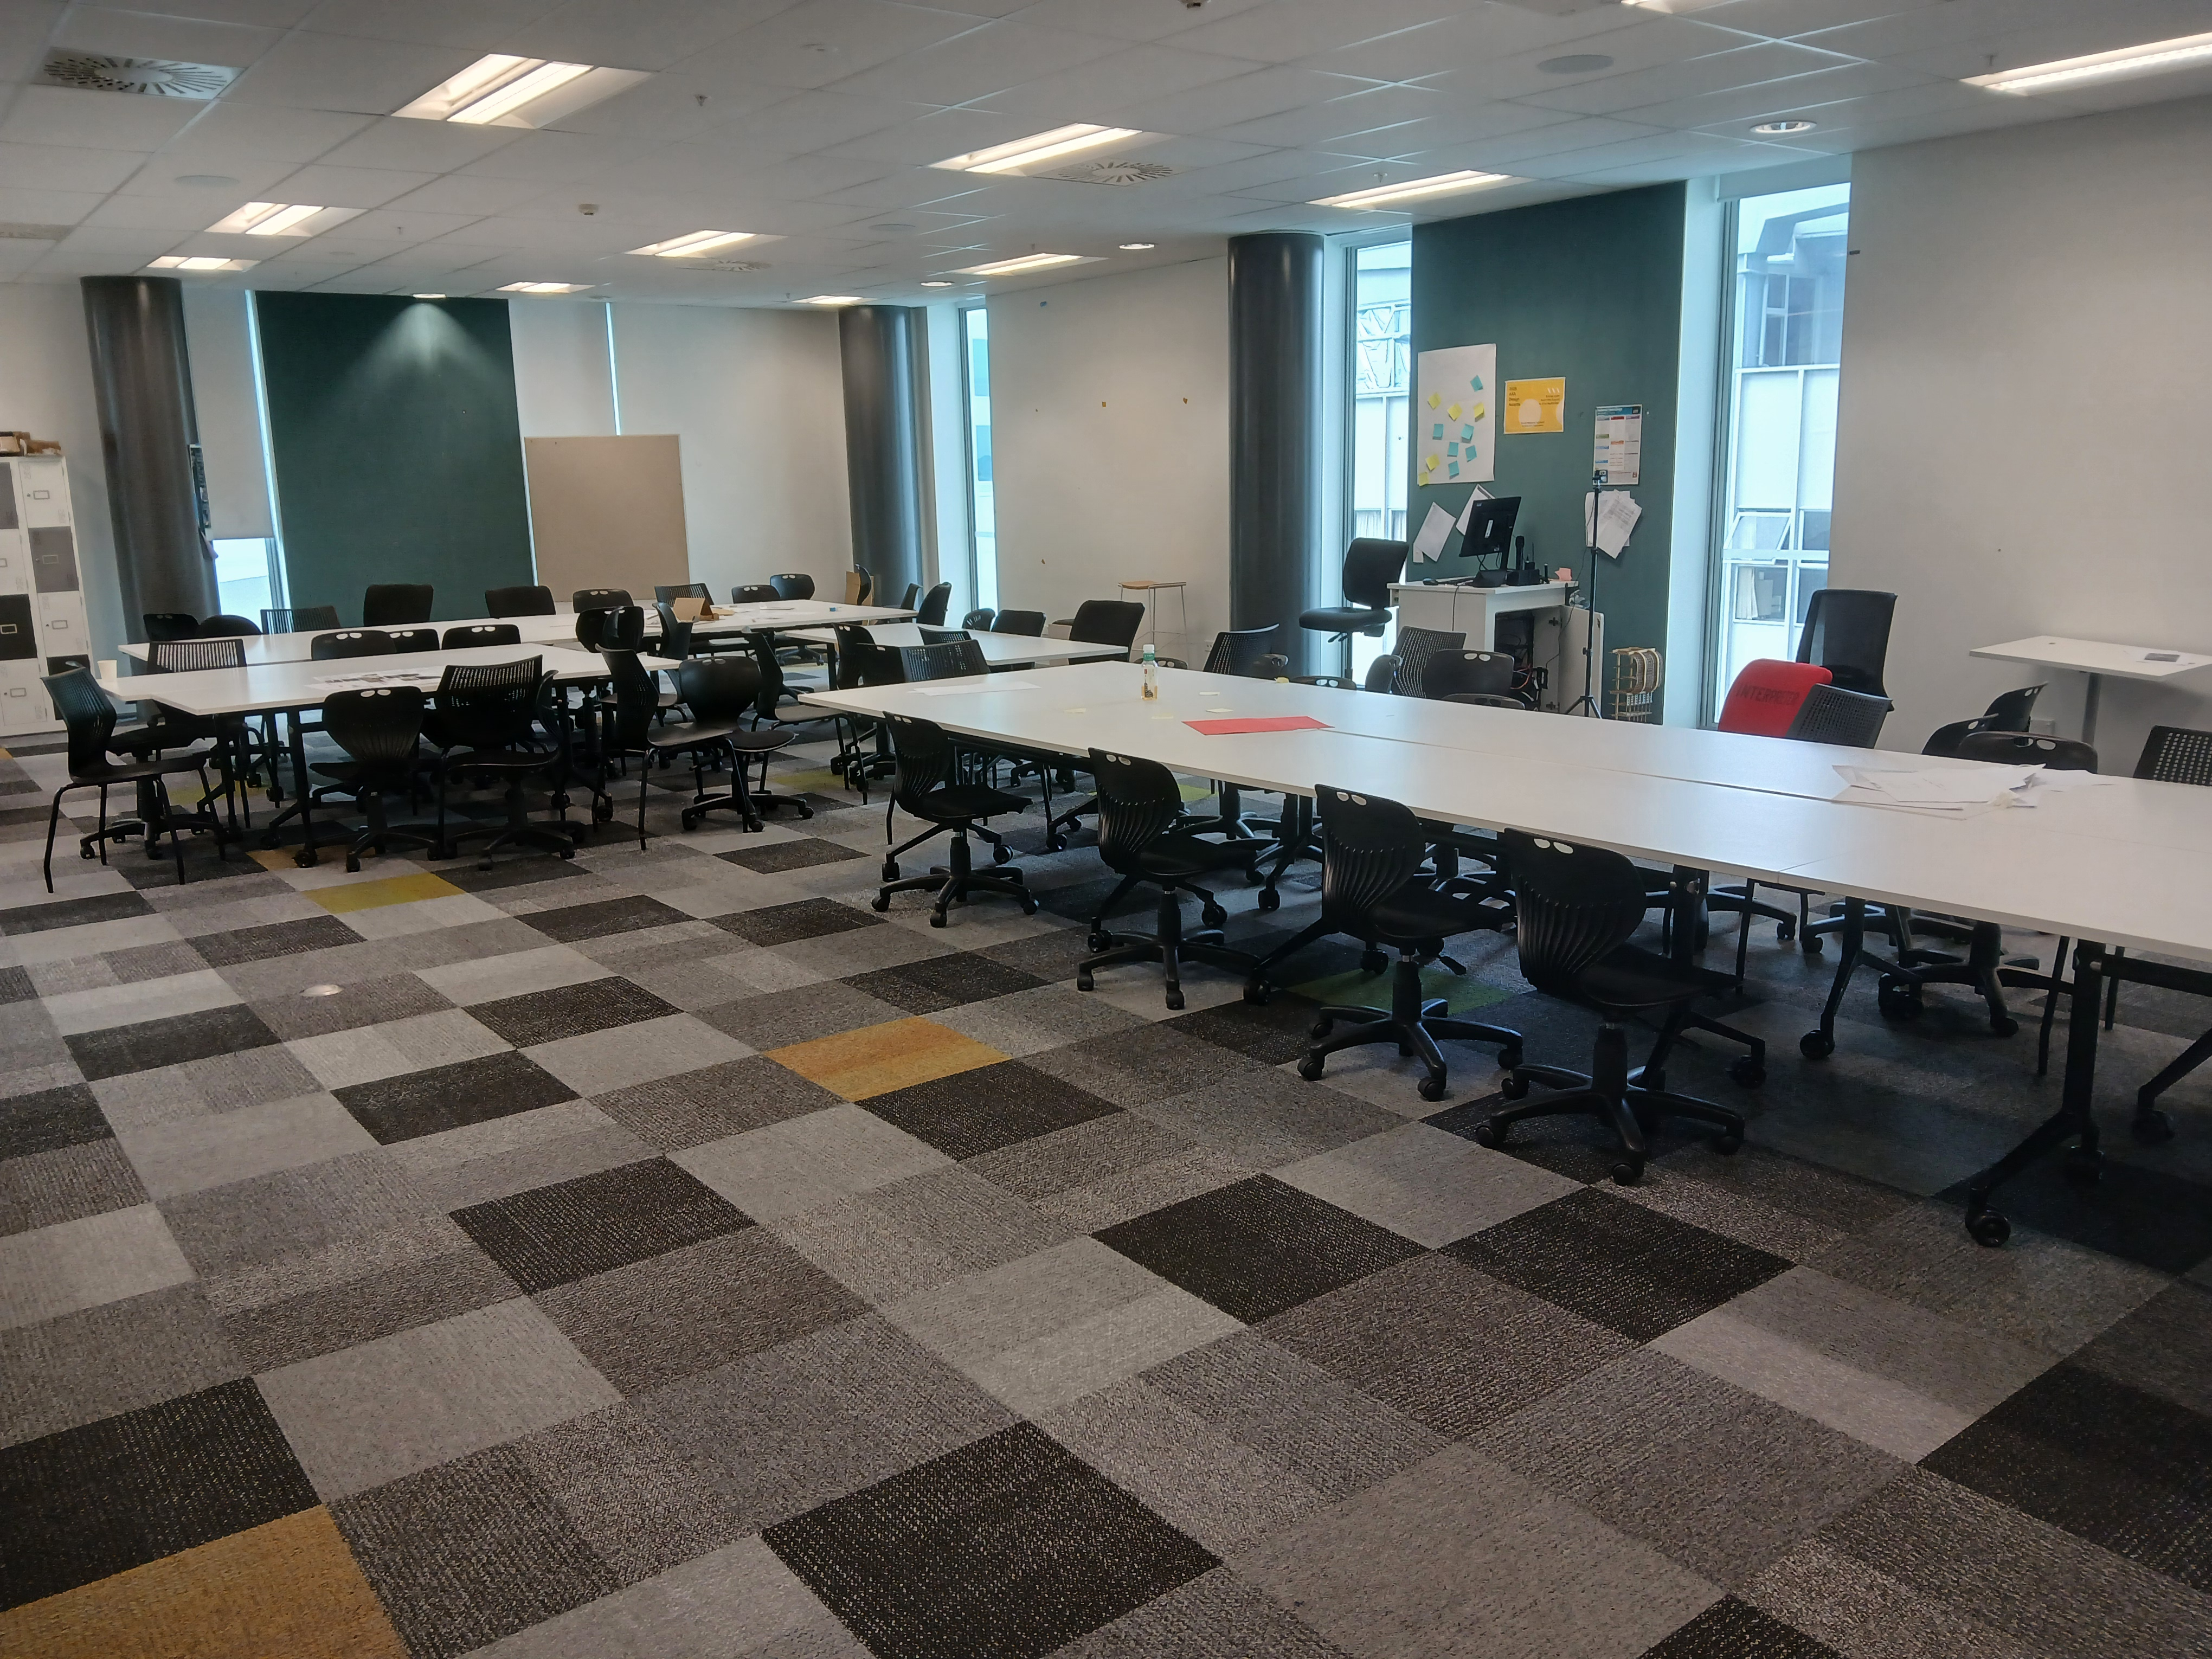
\includegraphics[alt={Figure 6.2},width=0.8\textwidth]{figures/F6-2.jpg}}
    \caption{Main Lecture Room \label{fig:6-2}}
\end{figure}

The very first session of the semester set the tone and flow for all the other sessions, which followed the same template. Students arrived within the first ten to twenty
minutes of the session while the teaching staff prepared the room and discussed the activities of the day. As it is tradition in almost all the Built Environments programs
(and many other programs at AUT), the lecture started with a Karakia, a traditional Māori prayer to open any social meeting or significant event, which Table \ref{tab:6-1}
shows in its Te Reo and English versions.

\begin{table}[]
\caption{Weekly Karakia}
\begin{tabularx}{\textwidth}{@{}cX@{}}
\textbf{Te Reo}          & \textbf{English}                                                                         \\ \midrule
Mauri oho                & Life force awaken.                                                                       \\
Mauri tū.                & Life force stand tall.                                                                   \\
Mauri ora ki a tātou.    & Life force all wellness, good health for all.                                            \\
Haumi e, Hui e! Tāiki e! & Join together, unite, the group is ready to progress for the purpose of coming together. \\ \bottomrule
\end{tabularx}
\label{tab:6-1}
\end{table}

Although it is a simple detail and a bit detached from the overall objectives of the observations, the Karakia became a constant reminder of the tone and mindset needed for
a successful experience in the course, and a tradition that reminded the students that they were entering a place meant for working together.

The first discussion during the introductory session was on tips and recommendations about how to handle the stress of the course, a very telling detail. Industry Project
is designed to be a complex course, that complexity is what allows the students to gain experience in a project close to what is found on the industry, but it also causes
a lot of friction for the students who are trying to manage all the academical requirements of the course.

The discussion asked the students to think on the requirements of the course from two views: the individual responsibilities to complete each of the deliveries and the
contribution there are giving to the shared project. The lecturer stated very clear recommendation for this purpose:

\begin{itemize}
    \item Be proactive with work, decisions and resources. Don't assume that everyone knows what is happening.
    \item Work together; the whole project cannot be finished by one person.
    \item Distribute and communicate. Remember that team management also needs time to be completed.
\end{itemize}

The biggest challenge of the project was that each of the disciplines represented in the group had a piece of the information and the expertise needed to complete it.
Communication and proper management were a key aspect to successfully propose a coherent solution. This was the core design of the course, and it was communicated to the
students from the very beginning.

The third theme of the first session was the issue of group assignation, a completely administrative tasks, but by far the most important activity, at least from the point
of view of the students. The composition of the groups tried to accommodate two students per group of each of the roles: \ac{AE}, \ac{CE}, \ac{CM} and \ac{QS}. The number
of students in each program did not allow to cover all spots, with an approximate ratio of two quantity surveyors and construction engineers per construction manager, and
only 3 \ac{AE} for all the groups. Figure \ref{fig:6-3} shows a simplified example of the distribution of roles used so that the available \ac{AE} and \ac{CM}
could be shared between different groups.

\begin{figure}
    \centering{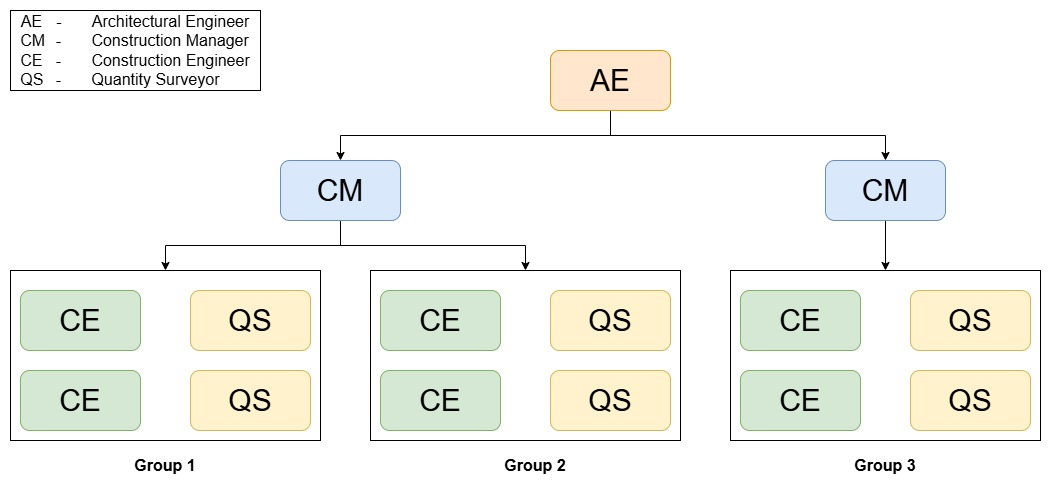
\includegraphics[alt={Figure 6.3},width=0.99\textwidth]{figures/F6-3.jpg}}
    \caption{Distribution of Shared Roles in the Groups \label{fig:6-3}}
\end{figure}

With this configuration, the groups were forced to share the work of the \ac{AE} and propose their own twists and takes on the common ideas present in the classroom. In
the same way, one \ac{CM} often had to coordinate the activities of at least two different groups. Intentional or not, this situation required a lot of effort to
coordinate the different roles in one group, and a disciplined flow of information from the \ac{AE} all the way to the \ac{CE} and the \ac{QS}. The situation matched
perfectly with the learning objectives of the course, albeit introducing a lot of administrative hurdles for the teaching staff.

For the observation protocol with \emph{WorkshopAR}, it meant that the cohesion of the groups was weaker than expected. Some students only needed to work with one specific group
and one set of overall goals, while others were required to constantly move between groups and solve different types of problems. Later it was observed that students
preferred to work with other people of their same role, blurring the boundaries between groups and creating a lot of horizontal communication between students.

\subsubsection{First Bonding Exercise \label{sec:6-4-1-1}}

After most of the students found their group, the rest of the time was used for what could be considered the first workshop activity of the semester. As with the
introduction, the main purpose of the workshop was to set the tone of the activities needed for the course and to create the correct mindset in the students about the
requirements of the project. The activity was also used as a way for each student to introduce themselves to the group.

As an icebreaker the lecturers proposed a simple discussion about the steps needed to bake a cake. The purpose was to create a debate in the group about quantity vs
quality in the development of the project and about procuring the proper ingredients for the chosen approach. The reflexion was that such a discussion must take place at
the beginning of their project, and highlighted the main activities that the group should be executing along the life cycle of the project:

\begin{itemize}
    \item Identify possible option to solve a problem.
    \item Discuss with the group all options and pick one.
    \item Work on the individual deliveries of the project based on the option selected.
    \item Communicate to the client the reasons behind the decision and the results of the work done.
\end{itemize}

This activity helped in creating observations of how different students approached that first contact with their group. Later, in the analysis process, those observations
would be used to discuss with the students possible scenarios in which \emph{WorkshopAR} could have helped in those activities, since it was not possible to intervene with the
software at that early stage of the course.

Team A was a good example of what was observed during this activity and, along the description of other teams in future sections, a good exercise to anchor the observations
to one easy-to-describe point of view that represents what was observed in other groups during the same activities.

Team A was mostly complete, all roles were present in the discussion except for one of the \ac{QS}. For most of the students, this was the first time meeting each other,
therefore their first conversation was not related at all to the activity, but focused on presentations, interchanging names, their current program (which was related to
their role) and contact information, mostly phone numbers, Instagram or Facebook.

Although the purpose of the activity was to formulate the main value proposition of the group, a rough idea of how the group would distinguish their proposal from the rest,
the discussion taking place in Team A centred more on trying to understand the premise of the project itself.

Those groups closer to the lecturers engaged more in the discussion about the value proposition, with constant interventions, questions and feedback from the lecturers.
Further away, groups like Team A defaulted more to idle chat or to those discussions about the exact work needed for the project, like the specific tasks they had to work
upon and what was supposed to be the purpose of their role. They were having problems identifying that information and a lot of questions started appearing among them.

The lecturers eventually spread around the room and talked with more groups, noticing the questions piling up. The general answer was that the project consisted in one
proposal from the group that had to be communicated to the client through the individual deliveries of each member. It was also remarked that more details about the project
would be discussed in the following sessions, and that all information about individual activities could be found in the \ac{LMS}.

From the activities and observations gathered during that first session, it was already possible to generate a couple of ideas about the design of the course that could
affect the development of \emph{WorkshopAR} or be the source of interesting data:

\begin{itemize}
    \item Mechanisms used by the students to navigate the complexity of the course.
    \item Differences in approaches and attitudes between those students engaged with the activities of the course and those falling behind.
    \item Mechanisms implemented by groups to manage the flow of information needed to fulfil the requirements of the project.
\end{itemize}

\subsubsection{Q\&A Sessions \label{sec:6-4-1-2}}

The initial reaction of confusion from almost all groups was expected, and the teaching staff had already prepared the second session of the course for a Q\&A session. The
idea was to keep up with the simulation, with the lecturers acting as the clients and providing information about the project, but it was also used to clarify details
about the deliveries and the marking criteria.

Figure \ref{fig:6-4} shows how the room was organised for the activity. This setup is relevant because it became the default configuration of the classroom for the rest of
the semester. For explicit Q\&A sessions and many of the workshops, the lecturers would ask the students to organize in this configuration and encourage students of the
same role to work together and exchange information. For the open work sessions, students would still use this setup to easily find other companions with the same role
when needed, compare work, and ask questions to see if someone had the answer.

\begin{figure}
    \centering{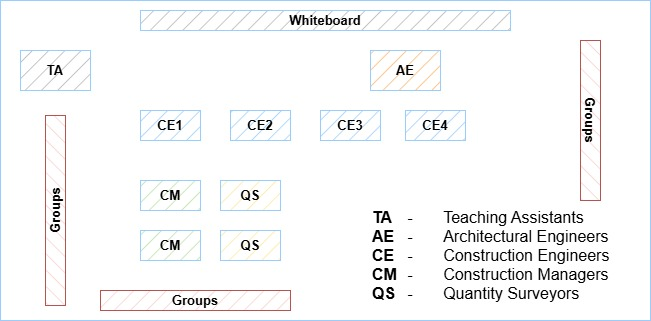
\includegraphics[alt={Figure 6.4},width=0.99\textwidth]{figures/F6-4.jpg}}
    \caption{Distribution of roles during Q\&A sessions \label{fig:6-4}}
\end{figure}

Groups would still work together in the available spaces around these central tables, but movement would be constant, with students coming and going between groups and
approaching one of the role tables if in need of information.

Some other aspects of consideration about this configuration of the classroom. First, the centre-stage position of the \ac{AE}. Since there were only three students in this
role, between five and six groups (an average of 15 to 20 students) depended on the work and decisions of one of the \ac{AE}. The structure of the project also required for
information about the architectural proposal and design to be the first element to be ready, and all the other roles had to wait for this activity to be completed before
being able to start working on their own responsibilities. Additionally, any question or change to the proposal had to flow back to the \ac{AE}, and the response had to
come back the same way, creating a lot of overtime of just waiting for responses that may not even come back.

The second aspect of notice was the \ac{TA}. The \ac{TA} group was very large, eleven different assistants, at least 1 representing each role. Often, the responsibilities
of any \ac{TA} would be to help the groups during the open work sessions, answering questions about the project and giving quick feedback to any work in progress. Each
\ac{TA} would do his or her best to help the students, but since each role was represented in the team, it was common for a \ac{TA} to not have an answer at hand, finding
the need to refer the students to another \ac{TA} or to the lecturers. The students quickly found easier to approach the \ac{TA} table, ask their questions to everyone and
see who could answer from all the people present in the table.

The Q\&A activities established the main workflow for all the students, at least for the first milestone of the project. This configuration of the classroom highlighted
several elements in the development of the course activities that where not part of the initial design of the \emph{WorkshopAR}:

\begin{itemize}
    \item The crucial participation of the lecturers and the TA team in the workflow of the groups.
    \item The constant movement of students between groups.
    \item The initial central focus of getting information from the role tables and bringing it back to the groups.
\end{itemize}

\subsection{Intervention with \emph{WorkshopAR} \label{sec:6-4-2}}

During the introduction of the teaching staff in the first session, the lectures acknowledged and presented the research project to the students and the ongoing
observations taking place in parallel to their work. Given the complexities of the first couple of weeks, no further direct mention of the research was done, with the idea
of not adding up even more elements to the already congested list of things that the students had to take care of during those first weeks.

Regrettably, this meant that all the activities that could be classified as part of the first acquaintance and consolidation stage of groupwork \parencite{lowe_1982} were
only part of general observations, as described in the previous section, and no direct intervention with \emph{WorkshopAR} was done.

It was not completely impossible to gather some data and direct experiences with the tool about the first encounter process, though. Most of the data and feedback from
usability tests and observations about the profile and user anchor features can be found in section \ref{sec:5-2-1-2}, which are functionalities related to the
consolidation stage of the group. Additionally, an observation that took place later in week 6 offered relevant ideas for this scenario.

\subsubsection{Consolidation Stage \label{sec:6-4-2-1}}

The proper introduction and description of the observed group will be done later in Section \ref{sec:6.5.2}. For now, it is enough to mention that the group was asked to
interact with the profile creation and the user anchor once they created and joined a \emph{digital room}. They were directly asked to remember their experience during the
first two weeks of the semester and to try to imagine if something of what happened could have been different (not necessarily better) if \emph{WorkshopAR} would have been
available to them back then.

Some responses stood out from all the comments given by the students while they were looking around the \emph{digital room} and mostly playing with the telescopic gaze of
the user anchor once they found that feature. One of the students mentioned that having a digital space where all the members of the group could be represented and have a
presence would have been useful to create a sense of belonging to the group from the very beginning.

They quickly referred to the initial chaos of trying to find their group. Most of them only had the number of the group as a reference, very few knew each other, and even
if they did, there was a high chance they were not in the same group. One of the students commented that he ended up shouting his number until he found his other companions,
prompting giggles from the others who were remembering the scene. Although humorous, the students confessed that it was unnecessarily stressful, and that the only other
resource to find their group was a huge diagram in the \ac{LMS} that they were having problems interpreting (the same diagram used to create the simplified version of
Figure \ref{fig:6-3}).

The students related this anecdote to \emph{WorkshopAR} by noticing that they could personalise the colour of the user anchor (see Section \ref{sec:5-2-1-2}), and that the
selection palette (accidentally) resembled that of the diagram in the \ac{LMS}. The students commented that the use of colour plus the visual anchor in the \ac{AR} space
could have been used to quickly identify other group members or at least other similar roles, as the configuration of the classroom was asking them to gather with other
students of the same role.

This described functionality was outside the designed use case but reflected well the idea of using visual cues created by \ac{AR} to convey a sense of belonging or
identity in the group. A similar set of ideas were discussed about the information that could be displayed when interacting with the user and room anchor.

The second major discussion was an interesting set of ideas about the technology used by the students to establish first contact with their peers. Their comments reflected
well what was later identified in interviews with students: students preferred to first establish a proper channel of asynchronous communication and resort to more direct
contact only if it was needed. One of the students even commented that she did some \emph{stalking} of one of her companions in social media to see who she was working with.

\subsubsection{First Open Work Session \label{sec:6-4-2-2}}

Towards week four, it had become clear that the original methodology proposed for the observations had to be altered. The observation plan stated that students who wanted
to participate in the study could contact the researcher to schedule a session, plus they could have access to a space for the group and take all the time they needed for
the activity. No group was taking on the offer, basically because no group was working together outside of the classroom.

Each weekly session had at minimum one hour of open work for the groups, with some weeks being dedicated completely to open sessions. Students quickly found that they
could gather in the classroom, organise the work needed for the week and assign individual tasks to be completed outside the classroom, relying on communication tools for
quick questions and catch-ups. Since no group was working outside the classroom, the observations using \emph{WorkshopAR} had to take place during the weekly sessions,
which forced some changes to the protocol:

\begin{itemize}
    \item Interact with only one group at a time and to not take the whole time of the open work session, to not interrupt the work of the students too much.
    \item Minimise disruptions to other groups and to other activities of the classroom. This often meant using more discrete recording methods, relying mostly on audio
    recordings and the field notes of the researcher.
    \item A focus on testing specific interactions with \emph{WorkshopAR} rather than the initial proposal of a more unscripted access to the tool. This approach was
    quicker, could be slotted easier in any schedule of activities for a classroom session and would interrupt the work of students the least.
    \item Not targeting the same group several times in a row. Although a lot of the subsequently discussed data comes from the same group, mostly because they were happy
    to keep collaborating with the project, all observations were done in sessions with enough time in between and at different stages of the project, so that the process
    was not a burden to the students.
\end{itemize}

With these new considerations, the plan was now to pick which features to introduce or focus upon for an observation and to move questions and conversations to more
specific points. All the observations of the use of \emph{WorkshopAR} that follow will have the same structure:

\begin{enumerate}
    \item Let the students organise themselves and decide or discuss what are they going to focus on during the \emph{work session}.
    \item Introduce \emph{WorkshopAR}, either from the very beginning or just the focus features for the observation.
    \item Let the students explore the functionalities, with the researcher asking questions to prompt discussion or to guide the students to a particular interaction with
    the application. Gather and record observations.
\end{enumerate}

Initially, the group volunteering for an observation would move to a different table in one of the rooms which was more secluded from the rest, with the idea of being able
to talk and record without disrupting the other groups. It ended up not being a good idea, because moving between rooms took away time from the observation (and from the
student's work) and limited the group's access to the \ac{TA} group or from the lecturers.

The following observation was of Team B during week four. The team had four members during this activity, two \ac{QS}, one \ac{CE} and one \ac{CM}. The group decided that
the main objective of the session was to work on the first poster presentation, which will be detailed in the next section. For the observation, the proposal was to focus
on two interactions:

\begin{itemize}
    \item The \emph{digital room} configuration.
    \item The profile configuration and the user anchors.
\end{itemize}

\emph{WorkshopAR} was deployed on two different smartphones and given to the students, which meant that in practice only two students were interacting with the software at
the same time. All the students had their own laptops and were working on them when not directly interacting in the observation activity.

The first step was to create and configure the \emph{digital room}. One of the \ac{QS} took the initiative to be the host and quickly moved through the technical steps all
the way to the creation of the \emph{workspace}. Defining the session goal did not take a discussion at all, since it had been already established previously. The mention
of the goal setting did prompt the question: What would happen if the goal had not been discussed earlier?

The response was a bit vague; the group had a clear idea of what was the work needed for the session, but it was not clear for them when they took the decision of
dedicating the session to start working on the poster. The \ac{CM} did mention that the poster was the next deliverable, so there was no need to discuss what to do next,
it was mandatory to work on the poster, and a matter of focusing on their own individual responsibilities.

The \ac{CM} continued this train of thought, proposing the scenario that if the lecturers expected a more step-by-step type of meetings, more formal approach to the group
work, that would be his main responsibility, and it would be clearer, at least for his role, what to do in each session. For now, he was feeling a little lost.

Figure \ref{fig:6-5} shows the space used for the couple of observations that took the groups apart from the rest of the classroom. The setup of the table promoted a
behaviour that had already been seen during the usability test: the student tried to create a \emph{workspace} that fitted in the entire table, although it was not necessary, and
was struggling with the controls and had to stand up and move around to try and cover the whole table. She was not happy with the result and asked to restart the process
to create a better \emph{workspace}.

\begin{figure}
    \centering{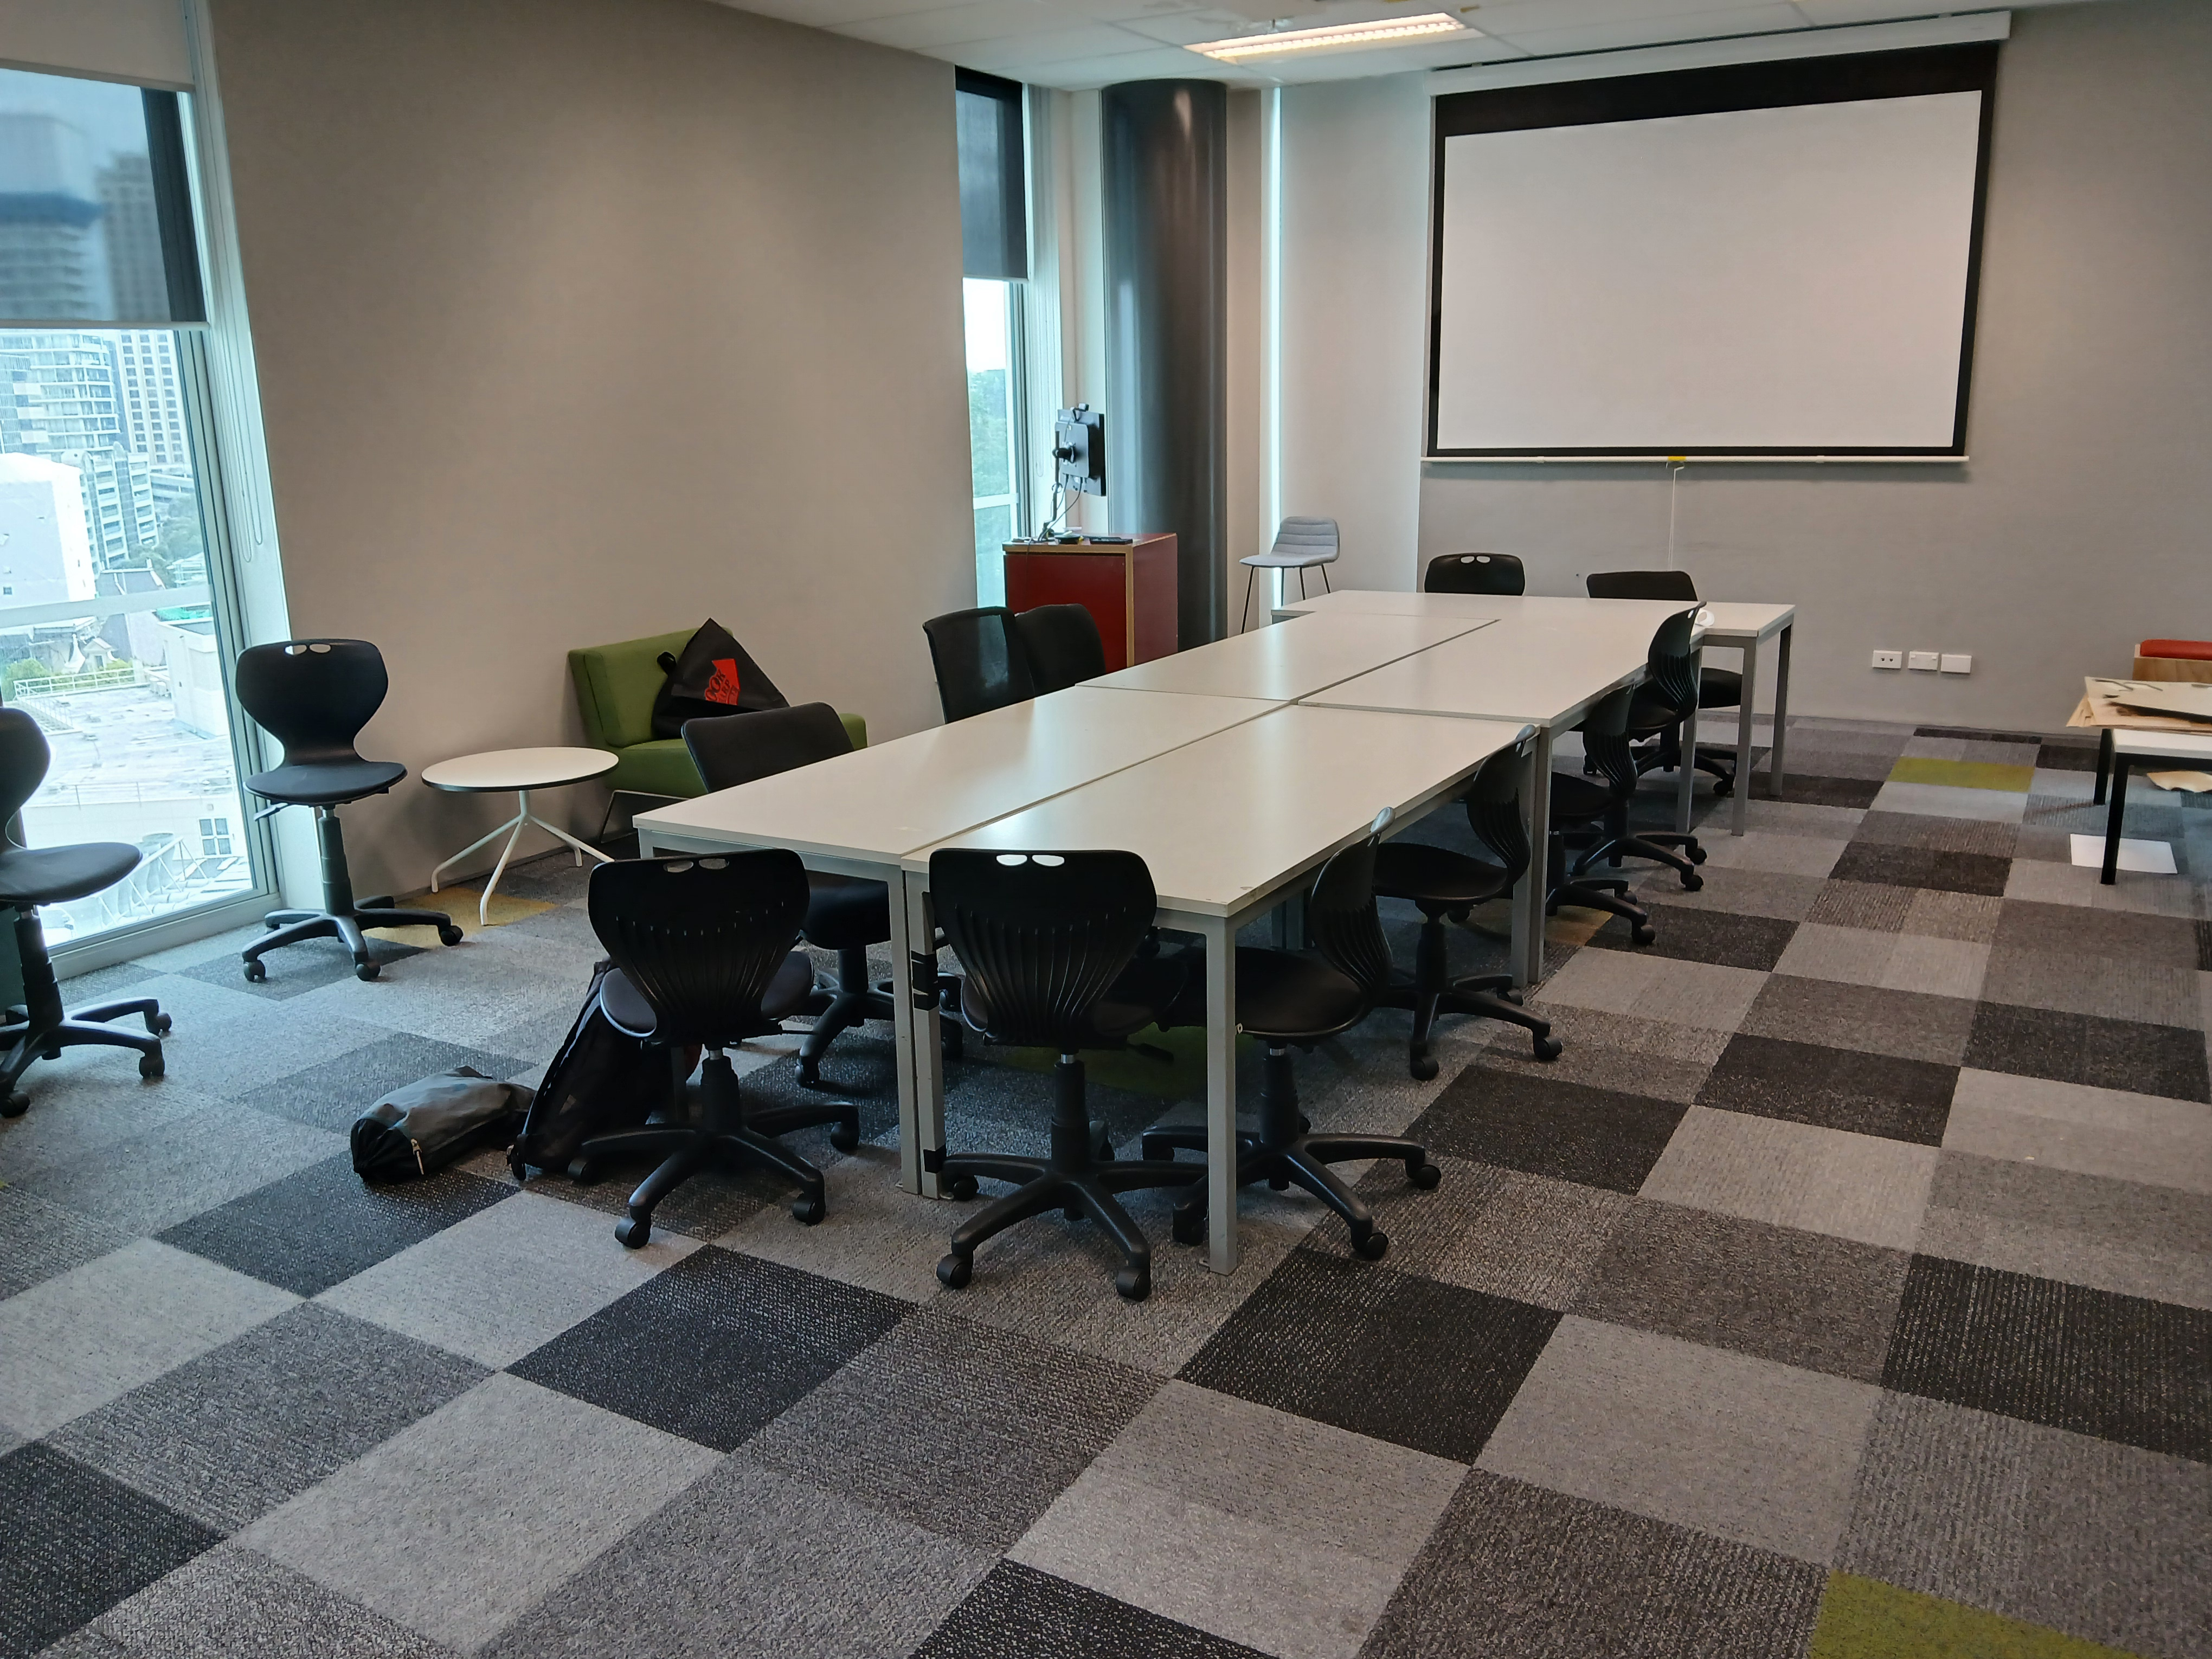
\includegraphics[alt={Figure 6.5},width=0.8\textwidth]{figures/F6-5.jpg}}
    \caption{Initial Space for Observations of \emph{WorkshopAR} \label{fig:6-5}}
\end{figure}

While repeating the creation of the \emph{digital room}, the student commented that the \ac{CM} should be the one in charge of the configuration process and handed the
mobile to him so he could do it. The situation prompted an intervening question: Should the same person always be the host? How would they organise the group to create and
configure the \emph{digital room}?

First, they proposed that it would make more sense if someone had that fixed responsibility but found little reasons to keep that idea when following the discussion
further. They argued that \emph{making} the \emph{digital room} should be a fast process and that the first person to arrive to the classroom should do it. This approach
was easier and would make the configuration time needed for the use of \emph{WorkshopAR} shorter.

The interactions with the user anchors also promoted some discussions about the use of the tool in the activities planned for the session. The students liked the idea of
the user anchor, they specially found amusing the \emph{goofy} look that the gaze gave to the whole visual, and suggested more elements of customisation beside colour,
like text, shapes, or animations. They also mentioned that the functionality was more suited for the first two weeks of the course, when it was more common to need
information about someone, like a name or a role, and was easier to fit the playfulness that the feature was promoting. For the work that the group was doing now, the
feature was rather useless, since they already knew each other and had other means of getting in contact if needed.

Other two important observations to mention that were not necessarily linked to the use of \emph{WorkshopAR}, but that were relevant to the dynamics were appearing in
almost every group:

First, when setting themselves up to start working, the \ac{CE} noticed that, based on the goal they had established of working on the poster, he had a lot of gaps in his
understanding of what he should be doing for the activity. The group tried to use the information found in the \ac{LMS} to clarify the situation, but it was not enough,
and a \ac{TA} had to intervene.

The second observation was that the work done by the students was very individual in nature. They were working together physically, often sharing comments and information,
but in the end each one concentrated in their own work. The \ac{CE} needed to clarify his doubts about the same poster all the others were working on, but because none of
his teammates shared his role, they did not have a clear idea either of what the \ac{CE} should be doing.

\subsection{Preliminary Analysis \label{sec:6-4-3}}

The first four weeks of work were a period of contextualisation and adjustments. Students were prepared to tackle a course that was known to be complex, and their first
concern was to untangle the complexity and start working on the project as soon as possible.

The first issue that the students found, one that the teaching staff had to quickly acknowledge, was a limited access to information. The \ac{LMS} was obscuring the
requirements of the project in between links and tons of external material, and the teaching staff had to explain and repeat several times the same information. Activities
like the Q\&A sessions and the constant access to the \ac{TA} staff helped the students to clarify any doubts, but those were resources that only the groups consistently
attending the classroom session had access to.

The interactions with Team B showed that using the structure that \emph{WorkshopAR} was proposing, especially for assigning goals and tasks, helped to incorporate those elements
to the organisation of the team. It was especially useful when the goals were not clear or had not been discussed enough. That was an exceptionally good behaviour promoted
by the application and aligned with the learning design proposed.

The observation protocol had to be adjusted, but that was part of the objectives established for the first weeks. It was good that a major issue was identified early and
that there was time to propose a solution.

The main functionality of \emph{WorkshopAR} was understood by the students but its immediate value for the project was not really seen. The main point of comparison so far
between \emph{WorkshopAR} and what other groups were doing was the creation of relationships by using the available technology. It was observed that most groups did not
think too much at first about the in-person communication needed to work and were primarily concerned with establishing points of communication that are asynchronous in
nature (WhatsApp, Teams, Facebook).

Students commented that they preferred to first establish a relation through social media and communication technologies and then step into face-to-face work for more
complex tasks. A quick analysis of works like \textcite{an_2006,robinson_2012} give some validity to this idea, showing that students prefer quick, simple communication
via their preferred apps, but appreciated more face-to-face work for more complex work.

\section{Weeks 5 to 9: Poster Presentation \label{sec:6-5}}

The work done by the students all the way to week nine focused on one single activity: the first poster presentation. This activity was individual; each student had 5
minutes to present their poster to the teaching staff. Despite the individual nature of the presentation, there were some key points that required group coordination:

\begin{itemize}
    \item Each group was associated with one of the three \ac{AE} working on the course, which meant that design proposals were shared among separate groups.
    \item Each group had to take a communal decision of the main or signature material to be use for construction (timber, concrete, etc.) and base the project on that
    decision.
    \item All groups had to present the same major topics in the poster: a design proposal, an analysis of the contextual factors of the project (legal, ecological and the
    community) and a preliminary analysis of costs.
\end{itemize}

To fulfil these criteria, information had to constantly flow from the \ac{AE}, who originally proposed the design, to the \ac{CE} and \ac{QS} who had to analyse the
proposal and build a construction plan, which often required going back to the \ac{AE} to clarify elements about the proposal or to offer feedback about the feasibility or
viability of some aspect of the design.

Managing this flow of information was the major challenge front he students at this stage and constituted the biggest instance of collaborative work observed in the course.
\ac{AE}, \ac{CE} and \ac{QS} had clear goals, and once the issues of coordination and communication were solved, students could work steadily towards their own poster. The
\ac{CM}, on the other hand, had a challenging time understanding their role in the group, and what was expected of them in the poster presentation.

The bulk of the observations for this section consisted in that: how different groups solved (or failed to solve) the information flow issues, how much they collaborated
inside and outside the group to finish their individual work and how \emph{WorkshopAR} was later introduced to try and help in those steps.

\subsection{General Observations \label{sec:6-5-1}}

Weeks five to nine represented the biggest instance of collaborative work observed through the entirety of the course. The poster presentation was an individual activity
but required group coordination for good final presentation. The group had to work together on the analysis of the proposed design, on basic decisions about the direction
of the project, on a coherent cost analysis and a consistent look or brand for the team across all aspects of the project. Each individual activity needed information from
the others, and there was a clear flow of information between roles.

At this point the groups consistently assisting and working on the classroom sessions had divided in two distinct categories:

\begin{itemize}
    \item Groups that collected all the information needed and were progressing in different areas of the presentation.
    \item Groups that had not been able to communicate well and had not gathered enough information to show any substantial progress.
\end{itemize}

The following general observations detail the dynamics of teams clearly showing on of these two characteristics. Following the new protocol, it was possible to observe
their work based on the plans they had for the session and later introduce \emph{WorkshopAR} to contrast how the tool changed or influence their approach to the proposed
goals.

In both cases, the teams were working in the central layout of the room, that is, the tables assigned for Q\&A activities and that represented the easier way to have
access to the information needed for the poster. The \ac{AE}s would normally work in that section of the room, which meant it was the best time to have a conversation with
them, as well as with other students or with the lecturers. It also showed how much the groups mixed and moved around the room during that data collection period and later
settled down to work in their individual assignments.

\subsubsection{A Bad Example: Team C \label{sec:6-5-1-1}}

Team C was represented only by two people, both in the role of \ac{QS}. By their own assessment, they were having a lot of problems finishing their individual posters
because they had no concrete information that could be translated into a cost calculation (the main objective of the \ac{QS} at this point). Their goal for the session was
to compare their work with others and advance in the creation of the poster.

When asked to elaborate on why they thought they were having so many problems completing their work, the answer was fast and clear: they had had little contact with the
rest of the team in the last weeks. They described the communication of the group as broken because there was always missing information or a lot of uncertainty when asking
anything through the group chat. Information was always provided at the last minute, and they had seen each other waiting without gaining any progress because there was no
response from one or more members of the team.

Groups had a lot of interactions between each other, and information did not only flow vertically between the different roles, but also horizontally between the groups.
Students were working around the limited access to the \ac{AE} by getting answers from their roles in other groups, adapting, or directly copying information among them.
Since Team C had only two members present, they were working near another group and interacting with their \ac{CE}, since their own \ac{CE} had never appeared in class and
the students themselves reported to had never seen him in person.

The situation was not the best for the group, but the students had managed to use different workarounds to get the information needed and progress with their work. The
structure of the project also allowed them to focus on their individual assignments and to not worry much about the lack of group cohesion, to the point that they were not
genuinely concerned about the work of their teammates. It was a situation that eliminated some of the stress but that ran in contradiction with the objective of the
project-based approach.

\subsubsection{A Good Example: Team D \label{sec:6-5-1-2}}

Team D had a \ac{CM}, a \ac{QS}, a \ac{CE} and one of the \ac{AE} was also directly working with them during this observation. The \ac{CE} was the most interested in
working next to the \ac{AE}, since he needed clarification about the technical aspects of the design, and ended up working more next to him rather than with his group. That
did not mean that the rest of the group was not participating, it was possible to observe that every time the \ac{CE} had new information, the \ac{CM} and the \ac{QS} would
quickly catch up and compare notes. If there were questions, the \ac{CE} would go back to the \ac{AE} and would try to find a quick answer, then everyone would go back and
work in their own laptops. Communication was short and to the point, collaboration was minimal, but it was efficient, and the \ac{QS} directly commented that she had
finished the biggest portion of her work during that session.

The horizontal flow of information was also seen in here; the lecturers would encourage the students to use some of the tables in the room so that all \ac{QS} or all
\ac{CM} would talk with each other and could clarify doubts about the deliveries. The students did not used those tables that much, but it was common to see students going
from one group to another with their tablets or laptops asking questions or interchanging information.

\subsection{Intervention with WorkshopAR \label{sec:6-5-2}}

The previous section showed the overall dynamics created in the groups for the competition of the first assignments, and the most relevant challenges around the flow of
information and the communication issues within the group. For the second intervention with \emph{WorkshopAR} the objectives for the observation were the following:

\begin{itemize}
    \item Introduce the play models to discuss the aspects of the project related to the design proposal or to any activity related to the physical aspects of the project.
    \item Introduce the annotations as a tool for communication and management of information.
    \item Introduce the debates to aid in the discussion and decision-making process of the group.
\end{itemize}

The annotation and debate features were still in an early stage of development, and the observations focused more on the interaction with play models, but it was possible
to show their main functionality with the objective of identifying what elements could be refined or added during the second iteration of development. Despite the crude
state of the functionalities, both annotations and debates were well received, and it was possible to gather direct interactions and feedback for those features.

The observations will follow Team C and D again, as introduced in the previous section. In both cases, \emph{WorkshopAR} was quickly introduced to them, the major controls were
shown, and the group was given time to explore the configuration of the tool. After that, the focus was on the objective features.

\subsubsection{Annotations and Debate Features \label{sec:6-5-2-1}}

Team C interacted the most with annotations, and after briefly testing other functionalities like the user anchors and the debates, they agreed that the annotation feature
was the one they could be using the most.

Their immediate comparison was to the tool Miro \footnote{\url{https://miro.com/}}, a whiteboard-like application that both students were using to organise their work and
to share ideas. They associated to the annotation feature the same ideas they could explore in Miro: a repository and visual representation of a project, helping at
activities like brainstorming and free association of ideas.

Given this comparison to Miro, they were more interested in exploring the relationships that could be created between annotations. They recommended that it could be useful
to have some way to make these relations explicit by adding connectors like arrows or chains between annotations. The association of the annotation to the physical space
did not strike them as relevant or charged with meaning, but they did select a nearby wall to group all the annotations they were creating and called it the \emph{ideas board}.

Team D, on the other hand, barely interacted with the annotations, with one of the students remarking that the feature could quickly be abused to be rude to someone or to
just clutter the space with rubbish. The idea of using another tool as a visual repository of ideas was discussed before the interaction with \emph{WorkshopAR}, but none of the
students at Team D used something for that purpose, and could have been the reason they did not related to the annotation feature as much as Team C.

For both teams, the idea of expanding the annotation feature with graphical elements other than text was also immediately discussed, especially if it could be possible to
access the camera or the photo storage of the phone.

\begin{figure}
    \centering{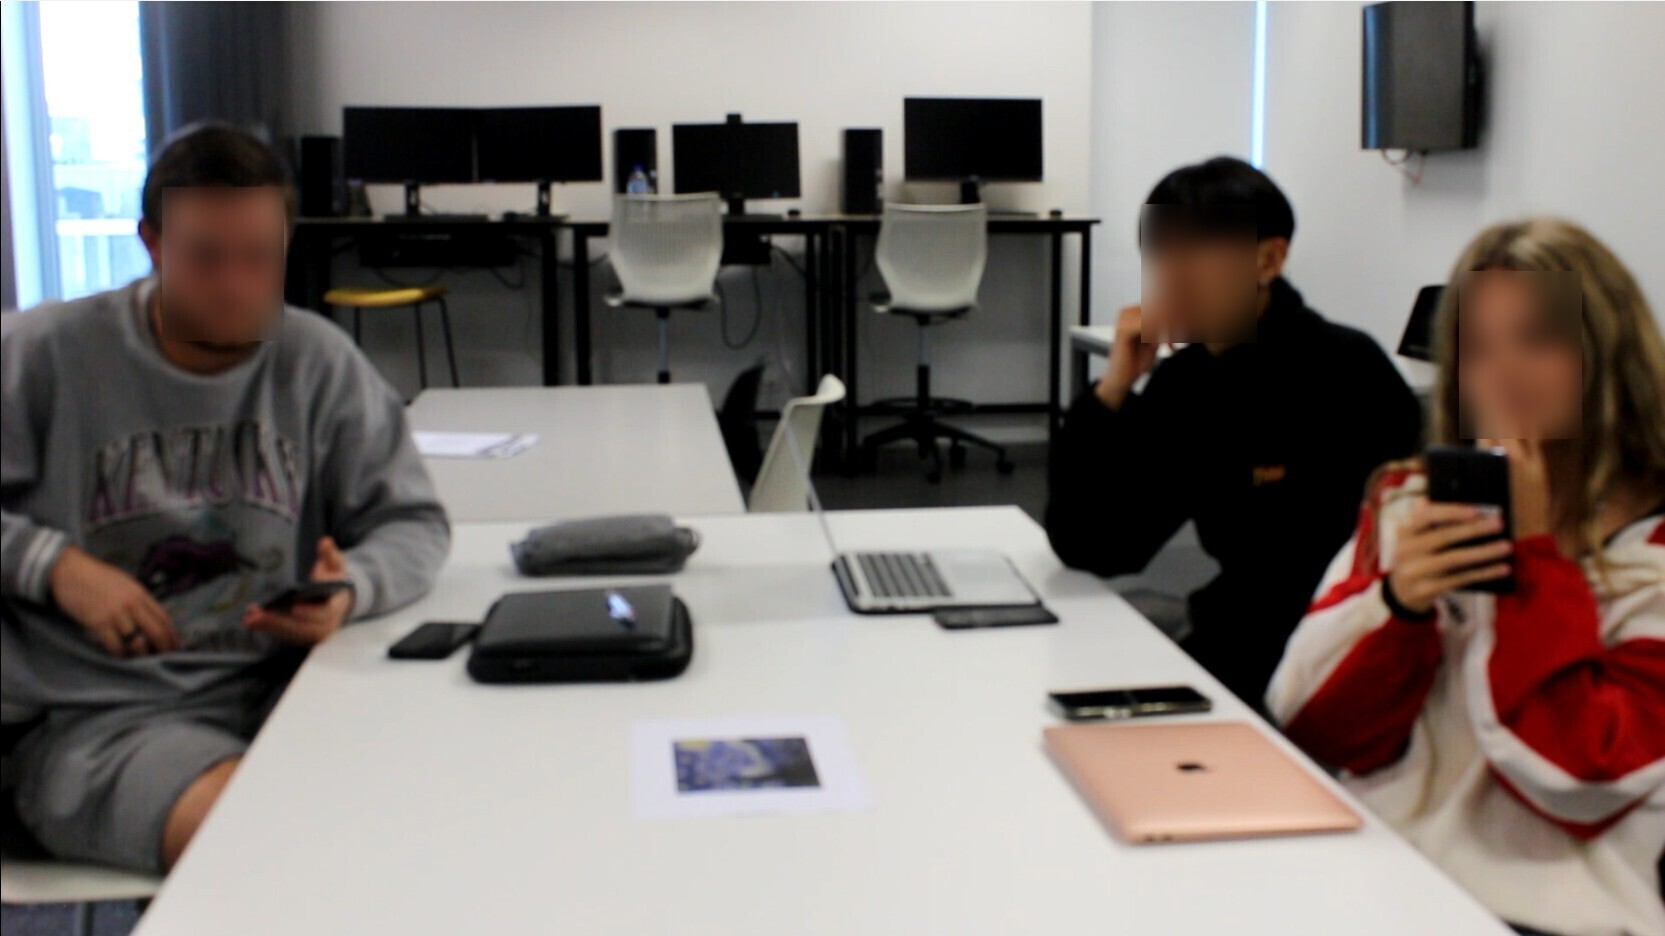
\includegraphics[alt={Figure 6.6},width=0.99\textwidth]{figures/F6-6.jpg}}
    \caption{Team D Working on the Room Configuration \label{fig:6-6}}
\end{figure}

Comments around the debate feature were the other way around. Team C did not have the need of using such a feature, since there was only two of them. They argued that such
a tool would make sense only for big teams, ten or more people, where it was possible to not know someone or for the necessity to manage the chaos of so many people trying
to decide something.

In contrast, the debate feature resonated the most with Team D. During the session, they had to take decisions regarding the construction material and some changes needed
to the design. While testing and exploring the functionality they even recreated a previous discussion about the selected construction material. Upon seeing that they had
four slots for the vote options, the \ac{AE} commented if it was worthy to discuss the addition of a third material. The other students, panicking, responded with a big no,
considering all the work they had already done with the original decision.

It was good that the tool promoted a deeper thought about the options of the debate and helped to flesh out the discussion, but it also showed that the users felt
obligated to configure all the options available, even if it was not necessary. This pointed to the need of tweaking the configuration of the debate. In the same line, it
was discussed that the configuration was taking too long for simple questions that could easily be asked aloud, echoing the comment of Team C that such a feature could be
better use in a bigger and newer team in needed of more control and management.

\subsubsection{Play Models \label{sec:6-5-2-2}}

Team C barely interacted with other features beside the annotations. They tested the interaction with play models, enough to offer some data about the controls and how the
improved control scheme was causing less problems in comparison to what was observed during the unstructured test. The group commented little about the tool and could not
relate the feature with their current work, as other students did in the past when interested in a functionality.

Team D offered a more telling interaction with the play models. The students tried for longer the actions related to the control scheme of the feature. They spent the most
time positioning different models around the space and sharing the interaction with their companions. They even took turns to interact with this feature the most.

It was possible to gather a lot of information about the interaction design, the UI, and the way to signal the protocol for shared models, as explored in section \ref{sec:5-2-1-3}.
The experience was not flawless, but the idea was clear to the students, and it was easy to identify and plan the needed adjustments that could be implemented for the
second iteration. The observations about how the tool integrated with the activities of the project was not as good.

This observation was a unique opportunity since both, an \ac{AE} and a \ac{CE} were present in the session, the two roles that could benefit the most from the play models.
Additionally, the group was communicating and understanding information about the architectural design, one of the intended use cases for the feature. The situation was
perfect and yet there were a lot of issues.

The first problem was that the tools the \ac{AE} and the \ac{CE} already used to create the architectural design were better suited to work on changes and faster to show
the results. Both students, when testing the tool, remarked that the play models could fit in the very initial discussion about the design, while gathering and drafting
ideas, but once the work started seriously, it was more productive to work and discuss over Sketch Up or AutoCAD. The \ac{AE} also mentioned how much of a problem it is to
get accustomed to a different control scheme when working in these types of 3D environments, and he personally would hate to jump from working with his mouse in the laptop
to trying some touchscreen control in the phone.

The second problem was just time itself. The concept of comparing the play models to playing with Lego blocks was mentioned several times and prompted the idea that the
feature would works very well with a playful attitude, when there was not yet a clear idea of what to do and the group is mostly generating ideas. Once the ideation phase
was done, it was important to move faster through the creation of actual material. The \ac{AE} also remarked that, with the configuration of groups that the course had
right now, it would be very difficult for him to recreate that ideation process with every group, which prompted him to just work alone and communicate his ideas in a
faster way.

The other students mirrored these thoughts. Being able to use the models to quicky visualise an idea or to communicate a design could work when there was not yet a
technical specification. Even with the possibility of integrating technical models into the tool, the conversation simply flowed faster and better by quickly discussing
things over their laptops and transmitting information and questions over instant messaging.

The area they thought had the most potential for a feature like the play models, especially if an external render could be integrated with the tool, would be in
communications with the client and the final presentation of their work, like with the poster presentation they were working on now. They mentioned that it would be an
extra layer of complexity for the presentation but would be an interesting and rather flashy tool to communicate the technical ideas of the project to the client in a way
that would offer an advantage over a poster or a written report.

\subsection{Preliminary Analysis \label{sec:6-5-3}}

The work done for the poster presentation represented the biggest instance in the course in which all the elements of collaborative work were present: students had to pool
their resources and agree on a solution. Work was interdependent, required planification, communication and coordination. Groups that were having a better time progressing
with the project were those that manage to establish a clear line of communication, learned to work with the needs and strengths of their team, were able to take decisions
fast and incorporate feedback when received. Groups having problems with the course where those that had a problem looking beyond the individual tasks required of each role,
had poor or non-existent channels of communication and were not using the spaces in the classroom to organise and check the status of their work.

So far, the students had interacted with the tools provided by WorkshopAR meant for team management and organization and with the interactions designed to help with
communication (annotation and debates) and with the co-creation activities of the project (the play models).

Figure \ref{fig:6-7} shows a simple comparison of how the four groups observed were dealing with the major activities identified at this point of the project. The
comparison is based on what was observed and reported by the students and their direct responses to how they would use \emph{WorkshopAR} in the same circumstances they were
at that moment.

\begin{figure}
    \centering{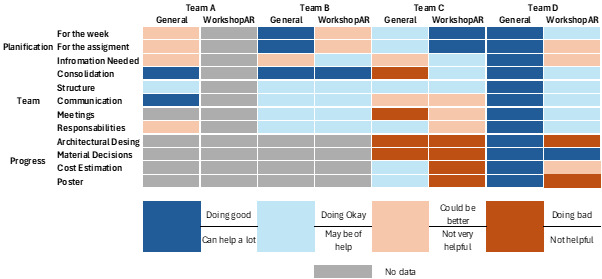
\includegraphics[alt={Figure 6.7},width=0.99\textwidth]{figures/F6-7.jpg}}
    \caption{Comparison Between the Reported State of a Group's Work and the Possible Benefits of the Use of \emph{WorkshopAR} \label{fig:6-7}}
\end{figure}

It was not possible to gather enough data from Team A to build a clear picture of how they would have used WorkshopAR during the first encounter activities or during their
work for the poster delivery. The main idea that was possible to extract from Team A was the importance that the flow of information had in the project and the challenges
experimented by the students to overcome it. Paired with the observations of the other teams, that division between groups properly managing the information issue and
those who could not was evident.

The first response of the students to \emph{WorkshopAR} was to that challenge of consolidating the group. The most consistent positive association was with management
activities, like organising the information of the participants and giving guidance on how to structure the activities of the day. Negative responses in this topic from
Team C and D derived directly from their situation during the observations. Team C had basically no team to manage, and Team D successfully formulated a working structure
for their group, making a direct use of the tools provided by \emph{WorkshopAR} less useful.

In both scenarios, \emph{WorkshopAR} only provided support for communication inside the team, and could not incorporate roles like the TA, the lecturers or other students
hoping between groups gathering information. This situation did not escape the design phase of the tool but was cut off in consideration of the scope of the research and
the initial set up of the observation process proposed. Interesting instances of collaboration were observed during these interactions, and this can be an interesting point
of expansion and refinement of the research in future work.

The response to the play models also made it clear that adjustments were needed. The major issues most students had with the tool were not much related with how it worked,
but how it could be incorporated in the activities they were focusing on. Team C was working on cost estimations since no other member of the group was with them,
therefore they found more use of the annotations and debates to organize ideas and manage discussion. Team D was in a better position to see the possible benefits of the
play models, but the tool did not offer much value at the stage their architectural design was.

For the next step in the execution of the case study and the development process running in parallel with \emph{WorkshopAR}, there were already several objectives in mind:

\begin{enumerate}
    \item Refine the interactions with the play models and identify how to integrate the activity better with the workflow of the students.
    \item Explore more the annotations and debate feature since they gathered the most attention from the students.
    \item Refine the way structure was presented to the students and allow for more flexible configurations.
\end{enumerate}

It was starting to be apparent that students were not so open to a work application, since they already had identified and integrated to their workflow all the tools they
considered necessary for their work. What resonated the most with them was the idea of a social space, and away to deal better with the issues of communication that were
taking place inside the classroom, and not so much outside of it.

\section{Weeks 10 to 13: Interim Client Report \label{sec:6-6}}